
\vspace{5 mm}

\begin{figure}[ht!]
\begin{center}
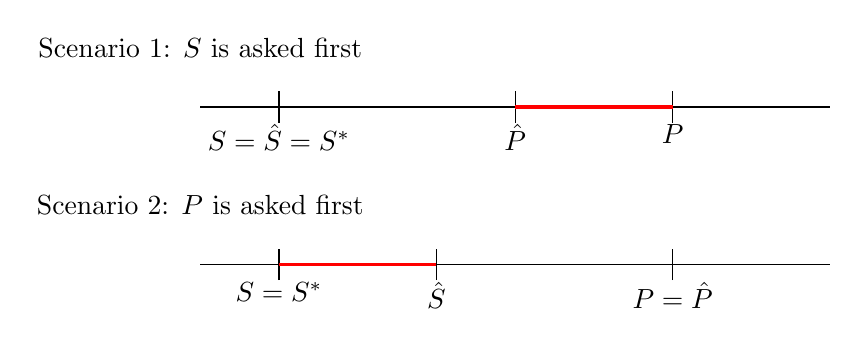
\begin{tikzpicture}

\draw ( -6,1) -- (-6,1) node [near start, below]{Scenario 1: $S$ is asked first};
\draw (-6,0) -- (2,0);
\draw ( 0,-0.2) -- ( 0,0.2) node [near start, below]{$P$}; 
\draw (-5,-0.2) -- (-5,0.2) node [near start, below]{$S = \hat{S} = S^*$};
\draw (-2,-0.2) -- (-2,0.2) node [near start, below]{$\hat{P}$};
\draw[red, very thick] (-2,0) -- (0,0) node [midway, above]{};


\draw ( -6,-1) -- (-6,-1) node [near start, below]{Scenario 2: $P$ is asked first};
\draw (-6,-2) -- (2,-2);
\draw ( 0,-2.2) -- ( 0,-1.8) node [near start, below]{$P = \hat{P}$}; 
\draw (-5,-2.2) -- (-5,-1.8) node [near start, below]{$S = S^*$};
\draw (-3,-2.2) -- (-3,-1.8) node [near start, below]{$\hat{S}$};
\draw[red, very thick] (-5,-2) -- (-3,-2) node [midway, above]{};

\end{tikzpicture}
\end{center}
\caption{Illustration of the proposed Data Generating Mechanism for one respondent: $S$ 'True' self position, $P$ 'True' perceived party position, $\hat{S}$ reported self position, $\hat{P}$ reported party position.
In red the convergence bias. $S^*$ is the self position predicted from observables.}
\label{fig:DGP}
\end{figure}